% Unofficial University of Cambridge Poster Template
% https://github.com/andiac/gemini-cam
% a fork of https://github.com/anishathalye/gemini
% also refer to https://github.com/k4rtik/uchicago-poster

\documentclass[final]{beamer}

% ====================
% Packages
% ====================

\usepackage[T1]{fontenc}
\usepackage{lmodern}
\usepackage[orientation=portrait,size=a0,scale=1.0]{beamerposter}
\usetheme{gemini}
\usecolortheme{nott}
\usepackage{graphicx}
\usepackage{booktabs}
\usepackage{tikz}
\usepackage{pgfplots}
\pgfplotsset{compat=1.14}
\usepackage{anyfontsize}
\usepackage{pythonhighlight}

% ====================
% Lengths
% ====================

% If you have N columns, choose \sepwidth and \colwidth such that
% (N+1)*\sepwidth + N*\colwidth = \paperwidth
\newlength{\sepwidth}
\newlength{\colwidth}
\setlength{\sepwidth}{0.025\paperwidth}
\setlength{\colwidth}{0.45\paperwidth}

\newcommand{\separatorcolumn}{\begin{column}{\sepwidth}\end{column}}

% ====================
% Paths
% ====================
\graphicspath{ {./images/} }

% ====================
% Title
% ====================

\title{SeaIceRT: a python interface for a Delta-Eddington radiative transfer model}

\author{Andrew P. Barrett \inst{1} \and Julienne Stroeve \inst{2} \and Bonnie Light \inst{3} \and Donald Perovich \inst{4}}

\institute[shortinst]{
  \inst{1} National Snow and Ice Data Center
  \samelineand \inst{2} University of Manitoba
  \samelineand \inst{3} Applied Physics Laboratory, University of Washington
  \samelineand \inst{4} University of Dartmouth
}

% ====================
% Footer (optional)
% ====================

\footercontent{
  \href{https://github.com/andypbarrett/seaice\_radiative\_transfer}{https://github.com/andypbarrett/seaice\_radiative\_transfer} \hfill
  Sea Ice Across Temporal and Spatial Scales, Bremerhavn, June 2023 \hfill
  \href{mailto:andrew.barrett@colorado.edu}{andrew.barrett@colorado.edu}}
% (can be left out to remove footer)


% ====================
% Logo (optional)
% ====================

% use this to include logos on the left and/or right side of the header:
\logoright{\includegraphics[height=7cm]{logos/NSIDC_logo_2018_poster.png}}
\logoleft{\includegraphics[height=7cm]{logos/cires_new_logo_large.png}}

% ====================
% Body
% ====================

\begin{document}

% Refer to https://github.com/k4rtik/uchicago-poster
% logo: https://www.cam.ac.uk/brand-resources/about-the-logo/logo-downloads
% \addtobeamertemplate{headline}{}
% {
%     \begin{tikzpicture}[remember picture,overlay]
%       \node [anchor=north west, inner sep=3cm] at ([xshift=-2.5cm,yshift=1.75cm]current page.north west)
%       {\includegraphics[height=7cm]{logos/unott-logo.eps}}; 
%     \end{tikzpicture}
% }

\begin{frame}[t,fragile]
\begin{columns}[t]
\separatorcolumn

\begin{column}{\colwidth}

  \begin{alertblock}{Summary}

    SeaIceRT is a python interface for the single column
    Delta-Eddington sea ice radiative transfer model from the Community Ice
    CodE (CICE) sea ice model used in the NCAR Community Earth System Model
    version 2 (CESM2). The python code provides a simple interface to the
    underlying FORTRAN radiative transfer model. Model parameters and forcing
    variables (ice thickness, snow depth and density, and melt pond depth) can
    be set and explored from an interactive environment such as ipython or
    Jupyter notebooks, as well as incorporated into python scripts to estimate
    under-ice light over periods of time, along transects or for grids for the
    Arctic Ocean. We demonstrate setting up and running the model for several
    transects collected during the MOSAiC cruise and for estimating
    phytoplankton bloom onset for the Arctic Ocean. We hope that the software
    package provides a framework for both simplifying and expanding access to
    these modelling tools. SeaIceRT is open source software. Documentation
    and code can be found at
    https://github.com/andypbarrett/seaice\_radiative\_transfer.

  \end{alertblock}

  \begin{block}{Motivation}

    \begin{figure}[h]
      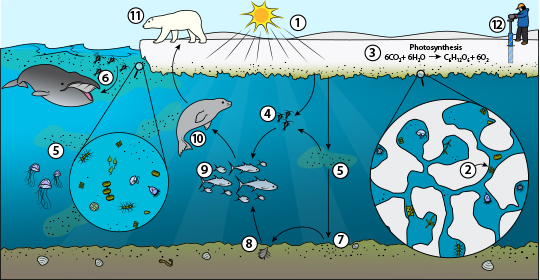
\includegraphics[width=0.75\textwidth]{ecosystemOverview-small}
      \caption{The Arctic Sea Ice Ecosystem https://askabiologist.asu.edu/explore/frozen-life \copyright Arizona Board of Regents ASU Ask A Biologist.}
    \end{figure}
    
    Sunlight transmitted through snow and sea ice to the upper ocean plays an
    important role in regulating biological activity in Polar regions,
    determining the timing of initiations of algal and phytoplankton blooms.
    Measurements of under-ice photosynthetically active radiation (PAR) are
    available from field campaigns and from autonomous buoys. However,
    understanding of the spatial distribution and time evolution of PAR for
    larger regions and over longer time periods requires estimates of light
    transmission through snow and sea ice from radiative transfer models. Even
    intensive and observation rich field campaigns such as MOSAiC can only
    collect measurements from a limited number of measurement points over
    selected periods of time. Radiative transfer models can be used to "fill
    in" gaps in the under ice light field, enabling observations of the
    atmosphere, snow and ice characteristics, oceanography and biology
    collected at distributed locations to be combined.

  \end{block}

  \begin{block}{The Delta-Eddington Radiative Transfer Model}

    This block catches your eye, so \textbf{important stuff} should probably go
    here.

    Curabitur eu libero vehicula, cursus est fringilla, luctus est. Morbi
    consectetur mauris quam, at finibus elit auctor ac. Aliquam erat volutpat.
    Aenean at nisl ut ex ullamcorper eleifend et eu augue. Aenean quis velit
    tristique odio convallis ultrices a ac odio.

    \begin{itemize}
      \item \textbf{Fusce dapibus tellus} vel tellus semper finibus. In
        consequat, nibh sed mattis luctus, augue diam fermentum lectus.
      \item \textbf{In euismod erat metus} non ex. Vestibulum luctus augue in
        mi condimentum, at sollicitudin lorem viverra.
      \item \textbf{Suspendisse vulputate} mauris vel placerat consectetur.
        Mauris semper, purus ac hendrerit molestie, elit mi dignissim odio, in
        suscipit felis sapien vel ex.
    \end{itemize}

    Aenean tincidunt risus eros, at gravida lorem sagittis vel. Vestibulum ante
    ipsum primis in faucibus orci luctus et ultrices posuere cubilia Curae.

  \end{block}

 \begin{block}{Nullam vel erat at velit convallis laoreet}

    Class aptent taciti sociosqu ad litora torquent per conubia nostra, per
    inceptos himenaeos. Phasellus libero enim, gravida sed erat sit amet,
    scelerisque congue diam. Fusce dapibus dui ut augue pulvinar iaculis.

    \begin{table}
      \centering
      \begin{tabular}{l r r c}
        \toprule
        \textbf{First column} & \textbf{Second column} & \textbf{Third column} & \textbf{Fourth} \\
        \midrule
        Foo & 13.37 & 384,394 & $\alpha$ \\
        Bar & 2.17 & 1,392 & $\beta$ \\
        Baz & 3.14 & 83,742 & $\delta$ \\
        Qux & 7.59 & 974 & $\gamma$ \\
        \bottomrule
      \end{tabular}
      \caption{A table caption.}
    \end{table}

    Donec quis posuere ligula. Nunc feugiat elit a mi malesuada consequat. Sed
    imperdiet augue ac nibh aliquet tristique. Aenean eu tortor vulputate,
    eleifend lorem in, dictum urna. Proin auctor ante in augue tincidunt
    tempor. Proin pellentesque vulputate odio, ac gravida nulla posuere
    efficitur. Aenean at velit vel dolor blandit molestie. Mauris laoreet
    commodo quam, non luctus nibh ullamcorper in. Class aptent taciti sociosqu
    ad litora torquent per conubia nostra, per inceptos himenaeos.

    Nulla varius finibus volutpat. Mauris molestie lorem tincidunt, iaculis
    libero at, gravida ante. Phasellus at felis eu neque suscipit suscipit.
    Integer ullamcorper, dui nec pretium ornare, urna dolor consequat libero,
    in feugiat elit lorem euismod lacus. Pellentesque sit amet dolor mollis,
    auctor urna non, tempus sem.

  \end{block}

\end{column}

\separatorcolumn

\begin{column}{\colwidth}

  \begin{exampleblock}{Running \pyth{SeaIceRT}}

    \pyth{SeaIceRT} is available from the https://github.com/andypbarrett/seaice\_radiative\_transfer github repository.
    Installation instructions along with software requirements are provided there.

    Once installed, SeaIceRT can be run in a Python interpretter, IPython or
    a Jupyter notebook.  I can also be included in other python scripts.  Example
    notebooks are provided in the \pyth{notebooks} folder.

    \vspace{10mm}
    
    \begin{python}[caption={A \pyth{Hello World} for \pyth{SeaIceRT}}]
      (seaice_radiative_transfer) nsidc-abarrett-442:seaicert$ ipython
      Python 3.7.6 | packaged by conda-forge | (default, Mar  5 2020, 15:27:18) 
      Type 'copyright', 'credits' or 'license' for more information
      IPython 7.17.0 -- An enhanced Interactive Python. Type '?' for help.

      In [1]: from ccsm3_sir_de import SeaIceRT
      In [2]: model = SeaIceRT()
      In [3]: model.run()
      In [4]: model.print_results()
      ----------------------------------------------------------------------
      CCSM3 Sea Ice Delta Eddington calculation
      ----------------------------------------------------------------------
      ----------------------------------------------------------------------
      Visible and near-ir direct and diffuse albedos
      Visible: 0.2 to 0.7 micrometers
      Near-IR: 0.7 to 5.0 micrometers
      ----------------------------------------------------------------------
      Albedo shortwave direct: 0.17
      Albedo shortwave diffuse: 0.19
      Albedo longwave direct: 0.06
      Albedo longwave diffuse: 0.06
 
      ----------------------------------------------------------------------
      Surface ansorption and Albedos
      ----------------------------------------------------------------------
      Visible solar absorbed by ocean: 27.5656681060791
      Near-IR absorbed by ocean: 0.0
      ----------------------------------------------------------------------
      Surface absorption ad albedos
      ----------------------------------------------------------------------
      Solar vs direct surface irradiance:   0.12 Wm-2
      
      ----------------------------------------------------------------------
      Snow/Sea ice transmitted flux (Tr fraction) and absorption (Q Wm-2)
      ----------------------------------------------------------------------
      Level      depth Tr_vs  Q_vs   Tr_ni  Q_ni   Q_total
      ----------------------------------------------------------------------
      0 surface                  26.88         68.01  94.89
                 0.000 1.0000        1.0000
      1 pond                     12.76         67.06  79.82
                 0.250 0.9494        0.0130
      2 pond                     12.08          0.93  13.01
                 0.500 0.8625        0.0002
      3 ice                       2.05          0.02   2.07
                 0.050 0.7888        0.0000
      4 ice                      10.84          0.00  10.84
                 0.375 0.6228        0.0000
      5 ice                       9.41          0.00   9.41
                 0.750 0.4730        0.0000
      6 ice                       6.78          0.00   6.78
                 1.125 0.3551        0.0000
      7 ice                       4.61          0.00   4.61
                 1.500 0.2612        0.0000
      8 ocean                    27.57          0.00  27.57
    \end{python}
    

  \end{exampleblock}

  \begin{block}{Fusce aliquam magna velit}

    Et rutrum ex euismod vel. Pellentesque ultricies, velit in fermentum
    vestibulum, lectus nisi pretium nibh, sit amet aliquam lectus augue vel
    velit. Suspendisse rhoncus massa porttitor augue feugiat molestie. Sed
    molestie ut orci nec malesuada. Sed ultricies feugiat est fringilla
    posuere.

    \begin{figure}
      \centering
      \begin{tikzpicture}
        \begin{axis}[
            scale only axis,
            no markers,
            domain=0:2*pi,
            samples=100,
            axis lines=center,
            axis line style={-},
            ticks=none]
          \addplot[red] {sin(deg(x))};
          \addplot[blue] {cos(deg(x))};
        \end{axis}
      \end{tikzpicture}
      \caption{Another figure caption.}
    \end{figure}

  \end{block}

  \begin{block}{Nam cursus consequat egestas}

    Nulla eget sem quam. Ut aliquam volutpat nisi vestibulum convallis. Nunc a
    lectus et eros facilisis hendrerit eu non urna. Interdum et malesuada fames
    ac ante \textit{ipsum primis} in faucibus. Etiam sit amet velit eget sem
    euismod tristique. Praesent enim erat, porta vel mattis sed, pharetra sed
    ipsum. Morbi commodo condimentum massa, \textit{tempus venenatis} massa
    hendrerit quis. Maecenas sed porta est. Praesent mollis interdum lectus,
    sit amet sollicitudin risus tincidunt non.

    Etiam sit amet tempus lorem, aliquet condimentum velit. Donec et nibh
    consequat, sagittis ex eget, dictum orci. Etiam quis semper ante. Ut eu
    mauris purus. Proin nec consectetur ligula. Mauris pretium molestie
    ullamcorper. Integer nisi neque, aliquet et odio non, sagittis porta justo.

    \begin{itemize}
      \item \textbf{Sed consequat} id ante vel efficitur. Praesent congue massa
        sed est scelerisque, elementum mollis augue iaculis.
        \begin{itemize}
          \item In sed est finibus, vulputate
            nunc gravida, pulvinar lorem. In maximus nunc dolor, sed auctor eros
            porttitor quis.
          \item Fusce ornare dignissim nisi. Nam sit amet risus vel lacus
            tempor tincidunt eu a arcu.
          \item Donec rhoncus vestibulum erat, quis aliquam leo
            gravida egestas.
        \end{itemize}
      \item \textbf{Sed luctus, elit sit amet} dictum maximus, diam dolor
        faucibus purus, sed lobortis justo erat id turpis.
      \item \textbf{Pellentesque facilisis dolor in leo} bibendum congue.
        Maecenas congue finibus justo, vitae eleifend urna facilisis at.
    \end{itemize}

  \end{block}

  
  \begin{block}{References}

    \nocite{*}
    \footnotesize{\bibliographystyle{plain}\bibliography{poster}}

  \end{block}

\end{column}
\separatorcolumn



\end{columns}
\end{frame}

\end{document}
